\begin{figure} [ht]
\begin{center}
% GNUPLOT: LaTeX picture with Postscript
\begingroup
  \makeatletter
  \providecommand\color[2][]{%
    \GenericError{(gnuplot) \space\space\space\@spaces}{%
      Package color not loaded in conjunction with
      terminal option `colourtext'%
    }{See the gnuplot documentation for explanation.%
    }{Either use 'blacktext' in gnuplot or load the package
      color.sty in LaTeX.}%
    \renewcommand\color[2][]{}%
  }%
  \providecommand\includegraphics[2][]{%
    \GenericError{(gnuplot) \space\space\space\@spaces}{%
      Package graphicx or graphics not loaded%
    }{See the gnuplot documentation for explanation.%
    }{The gnuplot epslatex terminal needs graphicx.sty or graphics.sty.}%
    \renewcommand\includegraphics[2][]{}%
  }%
  \providecommand\rotatebox[2]{#2}%
  \@ifundefined{ifGPcolor}{%
    \newif\ifGPcolor
    \GPcolortrue
  }{}%
  \@ifundefined{ifGPblacktext}{%
    \newif\ifGPblacktext
    \GPblacktexttrue
  }{}%
  % define a \g@addto@macro without @ in the name:
  \let\gplgaddtomacro\g@addto@macro
  % define empty templates for all commands taking text:
  \gdef\gplbacktext{}%
  \gdef\gplfronttext{}%
  \makeatother
  \ifGPblacktext
    % no textcolor at all
    \def\colorrgb#1{}%
    \def\colorgray#1{}%
  \else
    % gray or color?
    \ifGPcolor
      \def\colorrgb#1{\color[rgb]{#1}}%
      \def\colorgray#1{\color[gray]{#1}}%
      \expandafter\def\csname LTw\endcsname{\color{white}}%
      \expandafter\def\csname LTb\endcsname{\color{black}}%
      \expandafter\def\csname LTa\endcsname{\color{black}}%
      \expandafter\def\csname LT0\endcsname{\color[rgb]{1,0,0}}%
      \expandafter\def\csname LT1\endcsname{\color[rgb]{0,1,0}}%
      \expandafter\def\csname LT2\endcsname{\color[rgb]{0,0,1}}%
      \expandafter\def\csname LT3\endcsname{\color[rgb]{1,0,1}}%
      \expandafter\def\csname LT4\endcsname{\color[rgb]{0,1,1}}%
      \expandafter\def\csname LT5\endcsname{\color[rgb]{1,1,0}}%
      \expandafter\def\csname LT6\endcsname{\color[rgb]{0,0,0}}%
      \expandafter\def\csname LT7\endcsname{\color[rgb]{1,0.3,0}}%
      \expandafter\def\csname LT8\endcsname{\color[rgb]{0.5,0.5,0.5}}%
    \else
      % gray
      \def\colorrgb#1{\color{black}}%
      \def\colorgray#1{\color[gray]{#1}}%
      \expandafter\def\csname LTw\endcsname{\color{white}}%
      \expandafter\def\csname LTb\endcsname{\color{black}}%
      \expandafter\def\csname LTa\endcsname{\color{black}}%
      \expandafter\def\csname LT0\endcsname{\color{black}}%
      \expandafter\def\csname LT1\endcsname{\color{black}}%
      \expandafter\def\csname LT2\endcsname{\color{black}}%
      \expandafter\def\csname LT3\endcsname{\color{black}}%
      \expandafter\def\csname LT4\endcsname{\color{black}}%
      \expandafter\def\csname LT5\endcsname{\color{black}}%
      \expandafter\def\csname LT6\endcsname{\color{black}}%
      \expandafter\def\csname LT7\endcsname{\color{black}}%
      \expandafter\def\csname LT8\endcsname{\color{black}}%
    \fi
  \fi
    \setlength{\unitlength}{0.0500bp}%
    \ifx\gptboxheight\undefined%
      \newlength{\gptboxheight}%
      \newlength{\gptboxwidth}%
      \newsavebox{\gptboxtext}%
    \fi%
    \setlength{\fboxrule}{0.5pt}%
    \setlength{\fboxsep}{1pt}%
    \definecolor{tbcol}{rgb}{1,1,1}%
\begin{picture}(7200.00,5040.00)%
    \gplgaddtomacro\gplbacktext{%
      \csname LTb\endcsname%%
      \put(814,704){\makebox(0,0)[r]{\strut{}$0$}}%
      \put(814,1229){\makebox(0,0)[r]{\strut{}$0.2$}}%
      \put(814,1754){\makebox(0,0)[r]{\strut{}$0.4$}}%
      \put(814,2279){\makebox(0,0)[r]{\strut{}$0.6$}}%
      \put(814,2804){\makebox(0,0)[r]{\strut{}$0.8$}}%
      \put(814,3329){\makebox(0,0)[r]{\strut{}$1$}}%
      \put(814,3854){\makebox(0,0)[r]{\strut{}$1.2$}}%
      \put(814,4379){\makebox(0,0)[r]{\strut{}$1.4$}}%
      \put(946,484){\makebox(0,0){\strut{}$0$}}%
      \put(1532,484){\makebox(0,0){\strut{}$5$}}%
      \put(2117,484){\makebox(0,0){\strut{}$10$}}%
      \put(2703,484){\makebox(0,0){\strut{}$15$}}%
      \put(3289,484){\makebox(0,0){\strut{}$20$}}%
      \put(3875,484){\makebox(0,0){\strut{}$25$}}%
      \put(4460,484){\makebox(0,0){\strut{}$30$}}%
      \put(5046,484){\makebox(0,0){\strut{}$35$}}%
      \put(5632,484){\makebox(0,0){\strut{}$40$}}%
      \put(6217,484){\makebox(0,0){\strut{}$45$}}%
      \put(6803,484){\makebox(0,0){\strut{}$50$}}%
    }%
    \gplgaddtomacro\gplfronttext{%
      \csname LTb\endcsname%%
      \put(5816,4206){\makebox(0,0)[r]{\strut{}3-TFT}}%
      \csname LTb\endcsname%%
      \put(5816,3986){\makebox(0,0)[r]{\strut{}2-TFT+D}}%
      \csname LTb\endcsname%%
      \put(5816,3766){\makebox(0,0)[r]{\strut{}2-TFT-E+D}}%
      \csname LTb\endcsname%%
      \put(5816,3546){\makebox(0,0)[r]{\strut{}2-TFT-E+C}}%
      \csname LTb\endcsname%%
      \put(209,2541){\rotatebox{-270.00}{\makebox(0,0){\strut{}Cooperation}}}%
      \put(3874,154){\makebox(0,0){\strut{}Round}}%
      \put(3874,4709){\makebox(0,0){\strut{}Average Cooperation by Round with Neighbourhood Voting}}%
    }%
    \gplbacktext
    \put(0,0){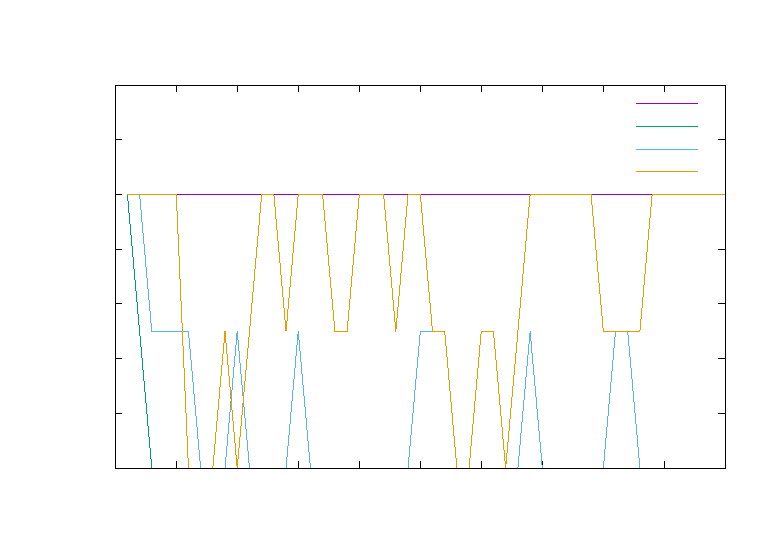
\includegraphics[width={360.00bp},height={252.00bp}]{neighbourhood}}%
    \gplfronttext
  \end{picture}%
\endgroup
 
\end {center}
\caption{Results from four 50 round tournaments with static agents
  with neighbourhood voting.  3-TFT refers to 3 tit-for-tat agents
  that start cooperating; they continue to cooperate.  2-TFT+D refers
  to two TFT agents with an agent that always defects; this
  quickly descends to no cooperation.  2-TFT-E+D refers to two
  TFT agents with 10\% exploration and an always defect agent;
  this system has some cooperations but mostly defects; note that it
  defects more than when there is pairwise voting.  2-TFT-E+C refers
  to two TFT agents with 10\% exploration and an agent that
  always cooperates; this cooperates about half the time, which is
  less than when there is pairwise voting.}
  \label{figStaticOneVote}
\end {figure}
